\documentclass[11pt,compress,t,notes=noshow, xcolor=table]{beamer}
\usepackage[]{graphicx}\usepackage[]{color}
% maxwidth is the original width if it is less than linewidth
% otherwise use linewidth (to make sure the graphics do not exceed the margin)
\makeatletter
\def\maxwidth{ %
  \ifdim\Gin@nat@width>\linewidth
    \linewidth
  \else
    \Gin@nat@width
  \fi
}
\makeatother

\newcommand{\citebutton}[2]{%
\beamergotobutton{\href{#2}{#1}}%
}

\newcommand{\blu}[1]{\textcolor{blue}{#1}}
\newcommand{\org}[1]{\textcolor{orange}{#1}}
\newcommand{\ques}{\textbf{\textcolor{red}{Question:  }}}
\newcommand{\questionssofar}{\begin{frame}\frametitle{Any questions?}\end{frame}}

\newcommand\warning{%
 \makebox[1.4em][c]{%
 \makebox[0pt][c]{\raisebox{.1em}{\scriptsize!}}%
 \makebox[0pt][c]{\color{red}\normalsize$\bigtriangleup$}}}%

\definecolor{fgcolor}{rgb}{0.345, 0.345, 0.345}
\newcommand{\hlnum}[1]{\textcolor[rgb]{0.686,0.059,0.569}{#1}}%
\newcommand{\hlstr}[1]{\textcolor[rgb]{0.192,0.494,0.8}{#1}}%
\newcommand{\hlcom}[1]{\textcolor[rgb]{0.678,0.584,0.686}{\textit{#1}}}%
\newcommand{\hlopt}[1]{\textcolor[rgb]{0,0,0}{#1}}%
\newcommand{\hlstd}[1]{\textcolor[rgb]{0.345,0.345,0.345}{#1}}%
\newcommand{\hlkwa}[1]{\textcolor[rgb]{0.161,0.373,0.58}{\textbf{#1}}}%
\newcommand{\hlkwb}[1]{\textcolor[rgb]{0.69,0.353,0.396}{#1}}%
\newcommand{\hlkwc}[1]{\textcolor[rgb]{0.333,0.667,0.333}{#1}}%
\newcommand{\hlkwd}[1]{\textcolor[rgb]{0.737,0.353,0.396}{\textbf{#1}}}%
\let\hlipl\hlkwb

\usepackage{framed}
\makeatletter
\newenvironment{kframe}{%
 \def\at@end@of@kframe{}%
 \ifinner\ifhmode%
  \def\at@end@of@kframe{\end{minipage}}%
  \begin{minipage}{\columnwidth}%
 \fi\fi%
 \def\FrameCommand##1{\hskip\@totalleftmargin \hskip-\fboxsep
 \colorbox{shadecolor}{##1}\hskip-\fboxsep
     % There is no \\@totalrightmargin, so:
     \hskip-\linewidth \hskip-\@totalleftmargin \hskip\columnwidth}%
 \MakeFramed {\advance\hsize-\width
   \@totalleftmargin\z@ \linewidth\hsize
   \@setminipage}}%
 {\par\unskip\endMakeFramed%
 \at@end@of@kframe}
\makeatother

\definecolor{shadecolor}{rgb}{.97, .97, .97}
\definecolor{messagecolor}{rgb}{0, 0, 0}
\definecolor{warningcolor}{rgb}{1, 0, 1}
\definecolor{errorcolor}{rgb}{1, 0, 0}
\newenvironment{knitrout}{}{} % an empty environment to be redefined in TeX

\usepackage{alltt}
\newcommand{\SweaveOpts}[1]{}  % do not interfere with LaTeX
\newcommand{\SweaveInput}[1]{} % because they are not real TeX commands
\newcommand{\Sexpr}[1]{}       % will only be parsed by R
\newcommand{\xmark}{\ding{55}}%


\usepackage[english]{babel}
\usepackage[utf8]{inputenc}

\usepackage{dsfont}
\usepackage{verbatim}
\usepackage{amsmath}
\usepackage{amsfonts}
\usepackage{amssymb}
\usepackage{bm}
\usepackage{csquotes}
\usepackage{multirow}
\usepackage{longtable}
\usepackage{booktabs}
\usepackage{enumerate}
\usepackage[absolute,overlay]{textpos}
\usepackage{psfrag}
\usepackage{algorithm}
\usepackage{algpseudocode}
\usepackage{eqnarray}
\usepackage{arydshln}
\usepackage{tabularx}
\usepackage{placeins}
\usepackage{tikz}
\usepackage{setspace}
\usepackage{colortbl}
\usepackage{mathtools}
\usepackage{wrapfig}
\usepackage{bm}
\usepackage{amsmath}
\usepackage{pifont}

\usetikzlibrary{shapes.multipart,shapes,arrows,automata,positioning,calc,chains,trees, shadows}
\tikzset{
  %Define standard arrow tip
  >=stealth',
  %Define style for boxes
  punkt/.style={
    rectangle,
    rounded corners,
    draw=black, very thick,
    text width=6.5em,
    minimum height=2em,
    text centered},
  % Define arrow style
  pil/.style={
    ->,
    thick,
    shorten <=2pt,
    shorten >=2pt,}
}

\tikzstyle{vec}=[draw, rectangle, fill = white, minimum width=5mm, minimum height=1cm, inner sep = 2pt]

\usepackage{subfig}

% Defines macros and environments
\usepackage{../../style/lmu-lecture}


\let\code=\texttt
\let\proglang=\textsf

\setkeys{Gin}{width=0.9\textwidth}

\setbeamertemplate{frametitle}{\expandafter\uppercase\expandafter\insertframetitle}

\usepackage{bbm}
% basic latex stuff
\newcommand{\pkg}[1]{{\fontseries{b}\selectfont #1}} %fontstyle for R packages
\newcommand{\lz}{\vspace{0.5cm}} %vertical space
\newcommand{\dlz}{\vspace{1cm}} %double vertical space
\newcommand{\oneliner}[1] % Oneliner for important statements
{\begin{block}{}\begin{center}\begin{Large}#1\end{Large}\end{center}\end{block}}


%new environments
\newenvironment{vbframe}  %frame with breaks and verbatim
{
 \begin{frame}[containsverbatim,allowframebreaks]
}
{
\end{frame}
}

\newenvironment{vframe}  %frame with verbatim without breaks (to avoid numbering one slided frames)
{
 \begin{frame}[containsverbatim]
}
{
\end{frame}
}

\newenvironment{blocki}[1]   % itemize block
{
 \begin{block}{#1}\begin{itemize}
}
{
\end{itemize}\end{block}
}

\newenvironment{fragileframe}[2]{  %fragile frame with framebreaks
\begin{frame}[allowframebreaks, fragile, environment = fragileframe]
\frametitle{#1}
#2}
{\end{frame}}


\newcommand{\myframe}[2]{  %short for frame with framebreaks
\begin{frame}[allowframebreaks]
\frametitle{#1}
#2
\end{frame}}

\newcommand{\remark}[1]{
  \textbf{Remark:} #1
}


\newenvironment{deleteframe}
{
\begingroup
\usebackgroundtemplate{
\includegraphics[width=\paperwidth,height=\paperheight]{../style/color/red.png}}
 \begin{frame}
}
{
\end{frame}
\endgroup
}
\newenvironment{simplifyframe}
{
\begingroup
\usebackgroundtemplate{
\includegraphics[width=\paperwidth,height=\paperheight]{../style/color/yellow.png}}
 \begin{frame}
}
{
\end{frame}
\endgroup
}\newenvironment{draftframe}
{
\begingroup
\usebackgroundtemplate{
\includegraphics[width=\paperwidth,height=\paperheight]{../style/color/green.jpg}}
 \begin{frame}
}
{
\end{frame}
\endgroup
}
% https://tex.stackexchange.com/a/261480: textcolor that works in mathmode
\makeatletter
\renewcommand*{\@textcolor}[3]{%
  \protect\leavevmode
  \begingroup
    \color#1{#2}#3%
  \endgroup
}
\makeatother





\input{../../latex-math/basic-math.tex}
\input{../../latex-math/basic-ml.tex}

\newcommand{\titlefigure}{figure/python.png}
\newcommand{\learninggoals}{
\item Understand the different package management systems
\item Be comfortable in settig up a python environment
\item Know how to make your work reproducible with Python}

\title{ML Basics}
% \author{}
\institute{\href{https://slds-lmu.github.io/lecture_dl4nlp/}{slds-lmu.github.io/lecture\_dl4nlp}}
\date{}

\begin{document}
\lecturechapter{Python Setup}
\lecture{Deep Learning for NLP}

% ------------------------------------------------------------------------------

\begin{vbframe}{0. Installation of Python}

\vfill

Python can be installed in many ways, e.g. by

	\begin{itemize}
		\item directly downloading it from \texttt{python.org}: \url{https://www.python.org/downloads/}
		\item downloading Miniconda: \url{https://docs.conda.io/en/latest/miniconda.html}
		\item installing Python via the Anaconda distribution: \url{https://docs.anaconda.com/anaconda/install/}
	\end{itemize}

\vfill

\end{vbframe}

% ------------------------------------------------------------------------------

\begin{vbframe}{0. Package management in Python}

\vfill

Unlike in R/RStudio (which you might be used to), package management in Python is a little more of a mess:  
There are \textit{two} package management systems:

\begin{itemize}
		\item \texttt{pip} (+ PyPi)
		\item \texttt{conda} (+ Anaconda repository)
\end{itemize}

\centering

\includegraphics[width=0.45\textwidth]{figure/conda.png}

\includegraphics[width=0.45\textwidth]{figure/pip.png}  

\vfill

\end{vbframe}

% ------------------------------------------------------------------------------

\begin{vbframe}{0. Package management in Python}
\vfill

\texttt{pip}
			
\begin{itemize}
		\item Installs packages from the \href{https://pypi.org/}{Python Package Index (PyPi)}
		\item Pip packages are source distributions (compiler needed) or wheels\footnote{}
		\item Installs dependencies in a recursive, serial loop
		\item Limited to Python software
		\item No built-in support for \textbf{virtual environments} (but possible)
		\item $>$ 150k packages available on PyPi
\end{itemize}

\vfill

\footnotesize $^1$tl;dr: wheels are smaller + install faster than a source distribution and do not require a compiler

\end{vbframe}

% ------------------------------------------------------------------------------

\begin{vbframe}{0. Package management in Python}

\vfill

\texttt{conda}

\begin{itemize}
		\item Installs packages from the \href{https://repo.anaconda.com/}{Anaconda repository}
		\item Conda packages are binaries, no need for compilers
		\item SAT solver to verify requirements of all packages
		\item Not limited to Python software
		\item Easier to create/manage \textbf{virtual environments}
		\item $\sim$ 1.5k packages available in the Anaconda repository
\end{itemize}

\vfill

\end{vbframe}

% ------------------------------------------------------------------------------

\begin{vbframe}{1. Python via the console}

\vfill

Start Python in Terminal / Console / Command Line
\vspace{-.2cm}
\begin{lstlisting}[language=bash]
python
\end{lstlisting}

Approximate result:\\

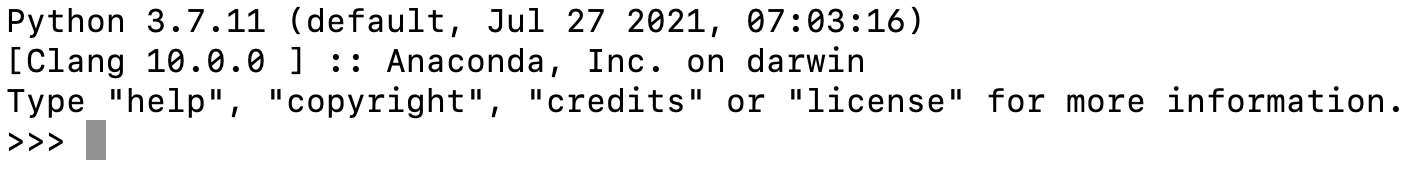
\includegraphics[width=0.95\textwidth]{figure/python_terminal.png}

Similar to R console:
\vspace{-.2cm}
\begin{lstlisting}[language=python]
1+1
\end{lstlisting}

Exit with Ctrl-D or
\vspace{-.2cm}
\begin{lstlisting}[language=python]
exit()
\end{lstlisting}

\vfill

\end{vbframe}

% ------------------------------------------------------------------------------

\begin{vbframe}{2. Anaconda}

\vfill

Anaconda is a widely used open-source distribution of Python: 
\url{https://www.anaconda.com}

\vspace{.5cm}

\centering

\includegraphics[width=0.5\textwidth]{figure/anaconda.png}

\vfill

\end{vbframe}

% ------------------------------------------------------------------------------

\begin{vbframe}{3. Miniconda}

\vfill

We recommend downloading and installing \textit{Miniconda}, since it

\begin{itemize}
	\item directly brings \texttt{conda} (as well as \texttt{pip})
	\item is a minimal installer (only the core parts, unlike Anaconda)
\end{itemize}

\centering

\includegraphics[width=0.8\textwidth]{figure/miniconda.png}

\tiny Source: \url{https://www.mrdbourke.com/get-your-computer-ready-for-machine-learning-using-anaconda-miniconda-and-conda/}

\vfill

\end{vbframe}

% ------------------------------------------------------------------------------

\begin{vbframe}{4. Spyder}

\vfill

\href{https://www.spyder-ide.org}{Spyder} is a complete IDE for Python (very similar to RStudio)

\centering

\includegraphics[width=0.5\textwidth]{figure/spyder.png}

\begin{itemize}
	\item directly comes with the Anaconda distribution
	\item can also be installed from \url{https://www.spyder-ide.org/}
\end{itemize}

\vfill

\end{vbframe}

% ------------------------------------------------------------------------------

\begin{vbframe}{5. Jupyter Notebooks/Lab}

\vfill

\begin{itemize}
	\item web application that lets you develop Python code in your browser
	\item combine code, text, images, and other media
	\item execute your code in smaller parts (cells)
	\item Useful for explorative analyses and for beginning stages of a project, where you need frequent feedback
\end{itemize}

\centering

\includegraphics[width=0.3\textwidth]{figure/jupyter.jpg}

\begin{lstlisting}[language=bash]
conda install jupyterlab
\end{lstlisting}

\vfill

\end{vbframe}

% ------------------------------------------------------------------------------

\begin{vbframe}{5. Jupyter Notebooks/Lab}

\vfill

Code cells vs. Markdown cells

\vspace{.2cm}


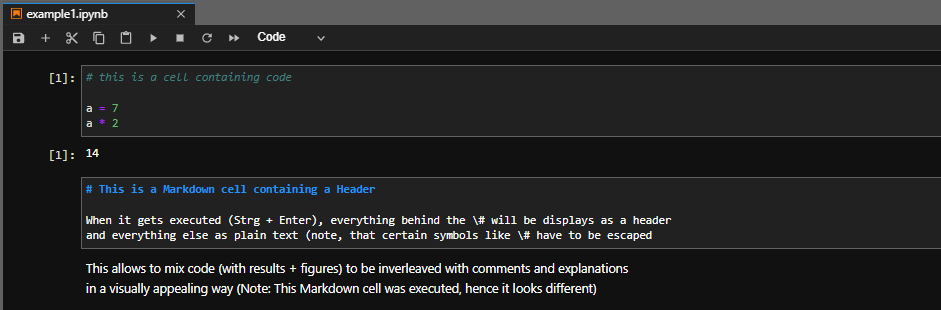
\includegraphics[width=.6\textwidth]{figure/jupyter1.png}

Useful for creating and changing figures quickly

\vspace{.2cm}

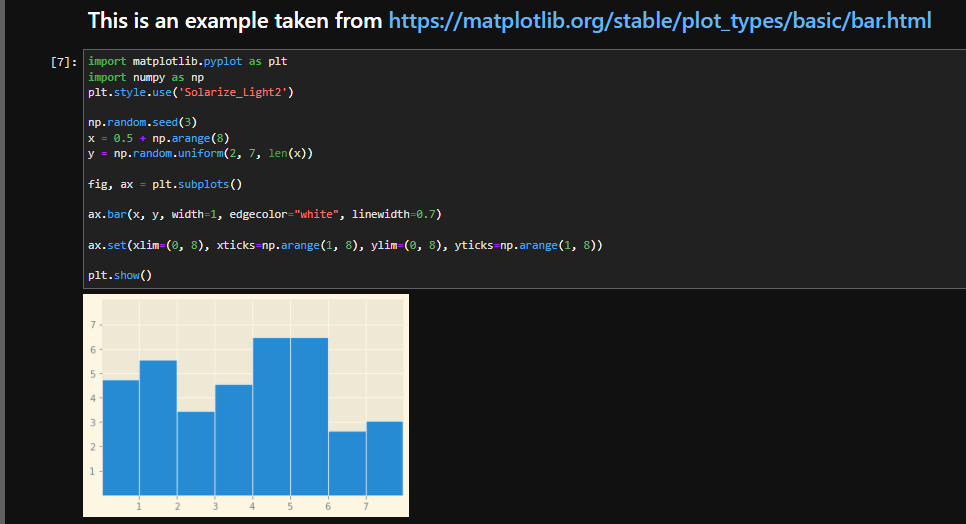
\includegraphics[width=.6\textwidth]{figure/jupyter2.png}

\vfill

\end{vbframe}

% ------------------------------------------------------------------------------

\begin{vbframe}{5. Jupyter Notebooks/Lab}

\vfill

\begin{itemize}
	\item When you click into a cell and you see your cursor, then you are in \textbf{Edit Mode}
	\item Write your Code/Explanations and execute with \texttt{Ctrl+Enter}
	\item Hit \texttt{Esc} $\rightarrow$ Cursor disappears, cell is still selected\\
  (you are in \textbf{Command mode} now)
	\item Now there are, among others, certain shortcuts available:
	\begin{itemize}
		\item \texttt{A} will insert a new cell \textit{above} the current one
    \item \texttt{B} will insert one \textit{below}
    \item \texttt{C} copies the selected cell
    \item \texttt{X} cuts the selected cell
    \item \texttt{V} pastes copied/cut cell below
    \item \texttt{M} switches the cell mode to \textit{Markdown}
    \item \texttt{Y} switches it to \textit{Code}
    \item \texttt{Up} selects cell above
    \item \texttt{Down} selects cell below
	\end{itemize}
\end{itemize}

\vfill

\end{vbframe}

% ------------------------------------------------------------------------------

\begin{vbframe}{6. Visual Studio Code}

	\vfill
	
	\begin{itemize}
		\item Widely used editor for many programming languages
		\item Main advantage: supports Jupyter Notebooks, takes care of setting up server
		\item install from \url{https://code.visualstudio.com/}
	\end{itemize}
	  
	
	\centering
	
\includegraphics[width=0.5\textwidth]{figure/vscode.png}
	
	\vfill
	
	\end{vbframe}

% ------------------------------------------------------------------------------

\begin{vbframe}{7. R-Studio}

\vfill

RStudio can also be used as an IDE for Python:  

\centering

\includegraphics[width=0.5\textwidth]{figure/rstudio.png}

\begin{itemize}
	\item Install the \texttt{reticulate} packages in R
	\item Select the desired Python interpreter at\\
  \texttt{Tools > Global Options > Python}
	\item \texttt{New File > Python Script}
\end{itemize}

\vfill

\end{vbframe}

% ------------------------------------------------------------------------------

% \begin{vbframe}{6. R-Studio}

% \vfill

% You can also use Python in conjunction with R Markdown\\
% (as you will observe quite often in our slides)

% \begin{lstlisting}[language=python]
% import pandas as pd

% x = pd.DataFrame({"a": [1,2,3,4],
%                   "b": ["c", "d", "e", "f"]})
% x
% \end{lstlisting}

% \vfill

% \end{vbframe}

% ------------------------------------------------------------------------------

\begin{vbframe}{8. Virtual Environments}

\vfill

Assume the following scenario:

\begin{itemize}
	\item We have two ongoing projects, \texttt{Project A} and \texttt{Project B}
	\item Both projects need some package \texttt{pkg\_xy}
	\item \texttt{Project A} needs \texttt{v1.2.0} while \texttt{Project B} requires \texttt{v2.1.3}
	\item What can we do about this?
\end{itemize}

\vspace{.2cm}

Solution: \textbf{Work with virtual environments}

% \begin{itemize}
% 	\item You can also tell RStudio to activate environments automatically by ticking the box at: 
% 	\item $\square$ \footnotesize \texttt{Automatically activate project-local Python environments}
% \end{itemize}

\vfill

\end{vbframe}

% ------------------------------------------------------------------------------

\begin{vbframe}{8. Virtual Environments}

\vfill

Virtual Environments allow you to 

\begin{itemize}
	\item have different entire version of Python running on your machine (\texttt{Python 2}, \texttt{Python 3.x}, \texttt{Python 3.y}, ..)
	\item maintain different versions of packages for your projects
\end{itemize}

\vspace{.3cm}

They can be created/activated/deactivated via

\begin{lstlisting}[language=python]
conda create --name some_name python=3.9
conda activate some_name
conda deactivate some_name
\end{lstlisting}

Useful commands: \href{https://docs.conda.io/projects/conda/en/4.6.0/_downloads/52a95608c49671267e40c689e0bc00ca/conda-cheatsheet.pdf}{Conda Cheat Sheet}

\vfill

\end{vbframe}

% ------------------------------------------------------------------------------

\begin{vbframe}{8. Virtual Environments}

\vfill

Different versions of Python

\vspace{.2cm}

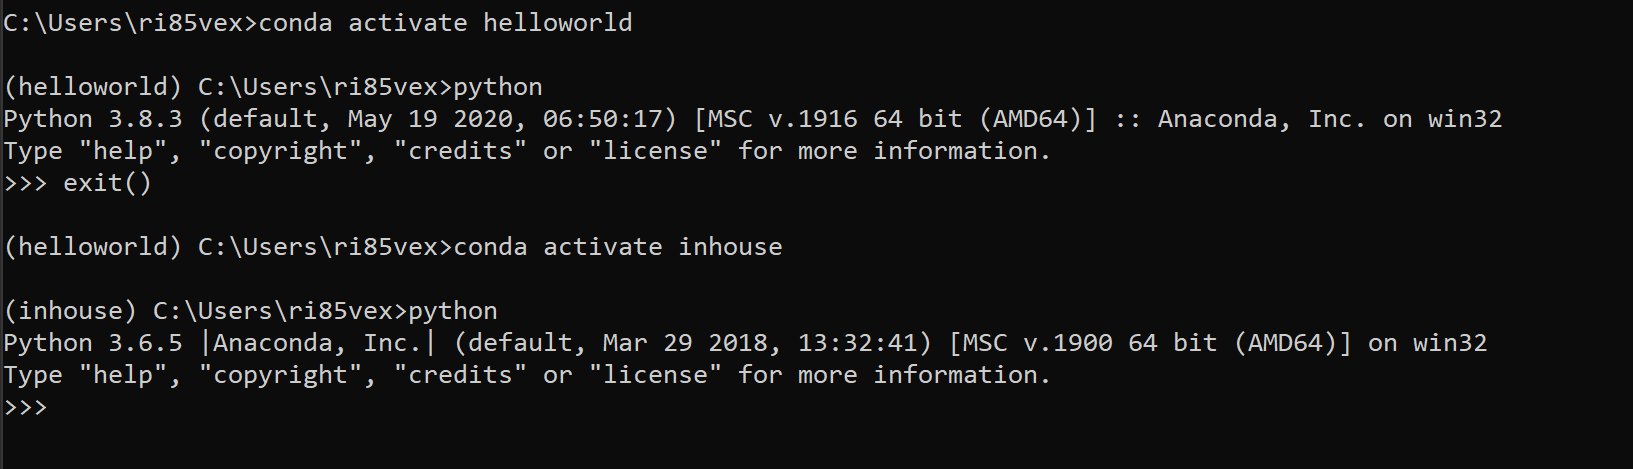
\includegraphics[width=.8\textwidth]{figure/envs.png}

Different (versions of) packages

\vspace{.2cm}

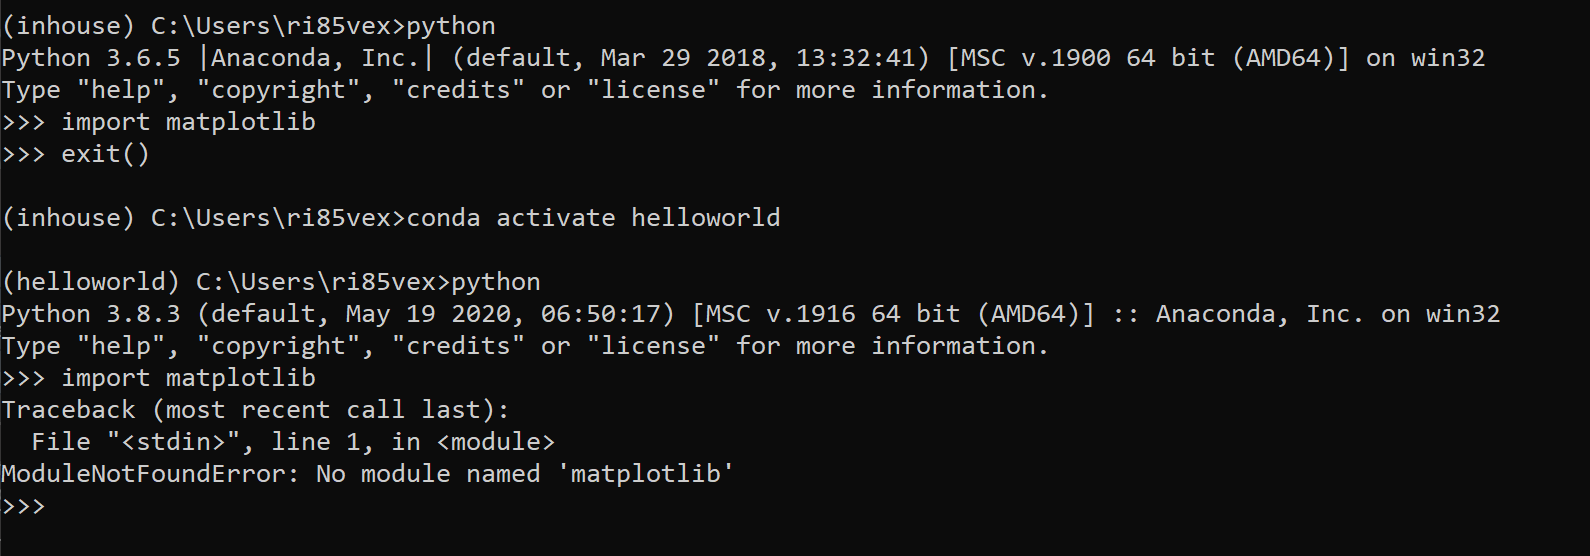
\includegraphics[width=.8\textwidth]{figure/envs2.png}

\vfill

\end{vbframe}

% ------------------------------------------------------------------------------

\begin{vbframe}{9. Managing packages}

\vfill

With \texttt{conda}:

\begin{lstlisting}[language=bash]
conda install pandas
conda install pandas==1.3.5
conda update pandas
conda remove pandas
conda list
\end{lstlisting}

With \texttt{pip}:

\begin{lstlisting}[language=bash]
pip install pandas
pip install pandas==1.3.5
pip install pandas --upgrade
pip uninstall pandas
pip freeze
\end{lstlisting}

\vfill

\end{vbframe}

% ------------------------------------------------------------------------------

\begin{vbframe}{9. Managing packages}

\vfill

Instruct \texttt{conda} which version you want to have installed:

\begin{itemize}
	\item Exact (1.3.5)
\begin{lstlisting}[language=bash]
conda install pandas==1.3.5
\end{lstlisting}
	\item Fuzzy (1.3.0, 1.3.1, etc.)
\begin{lstlisting}[language=bash]
conda install pandas==1.3
\end{lstlisting}
	\item Greater or equal (1.3.5 or higher)
\begin{lstlisting}[language=bash]
conda install "pandas>=1.3.5"
\end{lstlisting}
	\item OR (1.3.4 or 1.3.5)
\begin{lstlisting}[language=bash]
conda install "pandas==1.3.4|1.3.5"
\end{lstlisting}
	\item AND (1.3.3, 1.3.4, but not 1.4)
\begin{lstlisting}[language=bash]
conda install "pandas>=1.3.3,<1.4"
\end{lstlisting}

\end{itemize}

\vfill

\end{vbframe}

% ------------------------------------------------------------------------------

\begin{vbframe}{}

\vfill

Standardized way of sharing code requirements with others publicly across platforms:

\vspace{.3cm}

\begin{itemize}
	\item \texttt{environment.yml} (conda)
	\item \texttt{requirements.txt} (pip)
\end{itemize}

\vfill

\end{vbframe}

% ------------------------------------------------------------------------------

\begin{vbframe}{10. Reproducibility}

\vfill

\begin{itemize}
	\item Create an environment:\footnote{}\\
  (with specific Python version and some packages)
\begin{lstlisting}[language=bash,basicstyle=\tiny\ttfamily]
conda create -n my_env python=3.7 pandas numpy scikit-learn
\end{lstlisting}
	\item Activate the conda environment:
\begin{lstlisting}[language=bash]
conda activate my_env
\end{lstlisting}
	\item Export the specifications of your conda environment:
\begin{lstlisting}[language=bash]
conda env export > environment.yml
\end{lstlisting}
\end{itemize}

\vfill

\footnotesize $^3$\texttt{-n} is the short version of the \mbox{\texttt{-}}\texttt{-name} flag

\end{vbframe}

% ------------------------------------------------------------------------------

\begin{vbframe}{10. Reproducibility}

\vfill

Result (abbreviated to fit on the slide):

\scriptsize

\begin{lstlisting}[language=bash,basicstyle=\tiny\ttfamily]
name: my_env
channels:
  - defaults
dependencies:
  - blas=1.0=mkl
  - bottleneck=1.3.2=py37h2a96729_1
  - ...
  - numpy=1.21.2=py37hfca59bb_0
  - numpy-base=1.21.2=py37h0829f74_0
  - openssl=1.1.1l=h2bbff1b_0
  - packaging=21.3=pyhd3eb1b0_0
  - pandas=1.3.4=py37h6214cd6_0
  - pip=21.2.4=py37haa95532_0
  - pyparsing=3.0.4=pyhd3eb1b0_0
  - python=3.7.11=h6244533_0
  - python-dateutil=2.8.2=pyhd3eb1b0_0
  - pytz=2021.3=pyhd3eb1b0_0
  - scikit-learn=1.0.1=py37hf11a4ad_0
  - scipy=1.7.1=py37hbe87c03_2
  - ...
prefix: C:\Users\ri85vex\Miniconda3\envs\my_env
\end{lstlisting}

\vfill

\end{vbframe}

% ------------------------------------------------------------------------------

\begin{vbframe}{10. Reproducibility}

\vfill

\begin{itemize}
	\item \textit{Note 1:} As you can see, this also includes all sorts of packages that are automatically
  installed when creating an environment
	\item \textit{Note 2:} We observe some cryptic stuff after the version of each package 
  \item \textit{Note 3:} Those packages installed via pip are **also handled by this file** (see next slide)
  \item \textit{Note 4:} The \texttt{prefix} is ignored when using the \texttt{.yml}-file for creation.
  So you can simply delete it after the export.
\end{itemize}

\vfill

\end{vbframe}

% ------------------------------------------------------------------------------

\begin{vbframe}{10. Reproducibility}

\vfill

\begin{itemize}
	\item Install some package via \texttt{pip}:
		\begin{lstlisting}[language=bash]
pip install matplotlib
		\end{lstlisting}
	\item Result (abbreviated to fit on the slide):
		\begin{lstlisting}[language=bash,basicstyle=\tiny\ttfamily]
name: my_env
channels:
  - defaults
dependencies:
  - blas=1.0=mkl
  - bottleneck=1.3.2=py37h2a96729_1
  - ca-certificates=2021.10.26=haa95532_2
  - certifi=2021.10.8=py37haa95532_0
  - icc_rt=2019.0.0=h0cc432a_1
  - intel-openmp=2021.4.0=haa95532_3556
  - ...
  - pip:
    - cycler==0.11.0
    - fonttools==4.28.5
    - kiwisolver==1.3.2
    - matplotlib==3.5.1
    - pillow==9.0.0
prefix: C:\Users\ri85vex\Miniconda3\envs\my_env
		\end{lstlisting}
\end{itemize}

\vfill

\end{vbframe}

% ------------------------------------------------------------------------------

\begin{vbframe}{10. Reproducibility}

\vfill

\begin{itemize}
	\item Using the ``--from-history`` flag
		\begin{lstlisting}[language=bash]
conda env export --from-history > environment.yml
		\end{lstlisting}
	\item allows you to create a reduced version of the \texttt{.yml}-file containing only the packages (+ version) you explicitly installed (\textbf{via conda}):  
		\begin{lstlisting}[language=bash]
name: my_env
channels:
  - defaults
dependencies:
  - scikit-learn
  - numpy
  - python=3.7
  - pandas
prefix: C:\Users\ri85vex\Miniconda3\envs\my_env
		\end{lstlisting}
\end{itemize}

\vfill

\end{vbframe}

% ------------------------------------------------------------------------------

\begin{vbframe}{10. Reproducibility}

\vfill

\begin{itemize}
	\item Export specifications of the \texttt{pip} packages:
		\begin{lstlisting}[language=bash]
pip freeze > requirements.txt
		\end{lstlisting}
	\item Can be installed in a conda environment via:
		\begin{lstlisting}[language=bash]
pip install -r requirements.txt
		\end{lstlisting}
	\item \textbf{But}: Requiring others to execute these two steps will create a lot of work!
\end{itemize}

\vfill

\end{vbframe}

% ------------------------------------------------------------------------------

\begin{vbframe}{10. Reproducibility}

\vfill

\begin{itemize}
	\item Best practice: Create \texttt{.yml}-file manually
		\begin{lstlisting}[language=bash]
name: my_env
channels:
  - defaults
dependencies:
  - python=3.7.11
  - numpy=1.21.2
  - pandas=1.3.4
  - scikit-learn=1.0.1
  - pip=21.2.4
  - pip:
    # works for regular pip packages
    - matplotlib==2.0.0
    # also works for whole requirements-files:
    - -r requirements.txt
		\end{lstlisting}
	\item Finally: Create environment from \texttt{.yml}-file: 
		\begin{lstlisting}[language=bash]
conda env create -f environment.yml
		\end{lstlisting}
\end{itemize}

\vfill

\end{vbframe}

\endlecture
\end{document}
